% =====================================================================
%  HALAMAN SAMPUL
% =====================================================================
\begin{titlepage}
\centering
\singlespacing
\vspace*{0.3cm}
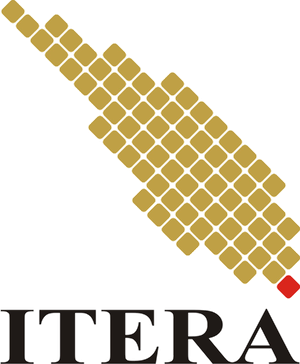
\includegraphics[width=2.4cm]{gambar/logo-itera.png}\par
\vspace{1cm}

{\bfseries\large TUGAS AKHIR\par}
{\bfseries\large LAPORAN TUGAS AKHIR\par}
{\small Bentuk 1: Penelitian Konvensional\par}
\vspace{1.2cm}

{\bfseries\fontsize{13}{16}\selectfont \judulTAkapital\par}
\ifpetunjuk{\scriptsize\itshape\color{abuisian}[Judul maksimal 16 kata]\par}\fi
\vspace{1.2cm}

{\small Diajukan sebagai luaran mata kuliah Tugas Akhir (IF25-40033)\par}
\vspace{1.2cm}

{\small\bfseries Disusun oleh:\par}
{\small \namaMhs\quad \nimMhs\par}
\vspace{0.6cm}
{\small Pembimbing: \pembimbing\par}

\vfill
{\small\bfseries
PROGRAM STUDI TEKNIK INFORMATIKA\par
FAKULTAS TEKNOLOGI INDUSTRI\par
INSTITUT TEKNOLOGI SUMATERA\par
LAMPUNG SELATAN\par}
{\small \tahunTA\par}
\vspace*{0.3cm}
\end{titlepage}
